\documentclass[a4paper,12pt]{article}

\usepackage[T1]{fontenc}
\usepackage[utf8]{inputenc}
\usepackage[italian]{babel}
\usepackage{eucal,enumitem}
\usepackage{graphicx}
\usepackage{amsmath,amssymb,amsthm}
\usepackage{tikz}
\usepackage{cancel} 
\usepackage{multicol}
\usepackage{color}
\usepackage{fancyhdr}
\usepackage{caption}

\begin{document}
Here a list of components to be used. 

\begin{figure}[h]
\centering
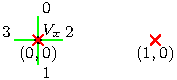
\includegraphics{nodeInfo}
\caption{Example of use of a generic node}
\label{nodeInfo} %Inserire sempre dopo caption
\end{figure}


\begin{figure}[h]
\centering
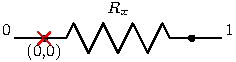
\includegraphics{resistorInfo}
\caption{Example of use of resistor}
\label{resistorInfo} %Inserire sempre dopo caption
\end{figure}

\begin{figure}[h]
\centering
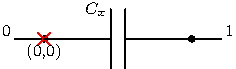
\includegraphics{capacitorInfo}
\caption{Example of use of capacitor}
\label{capaciorInfo} %Inserire sempre dopo caption
\end{figure}

\begin{figure}[h]
\centering
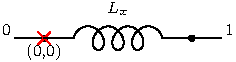
\includegraphics{inductorInfo}
\caption{Example of use of inductor}
\label{inductorInfo} %Inserire sempre dopo caption
\end{figure}

\begin{figure}[h]
\centering
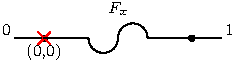
\includegraphics{fuseInfo}
\caption{Example of use of fuse}
\label{fuseInfo} %Inserire sempre dopo caption
\end{figure}

\begin{figure}[h]
\centering
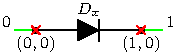
\includegraphics{diodeInfo}
\caption{Example of use of diode}
\label{diodeInfo} %Inserire sempre dopo caption
\end{figure}

\begin{figure}[h]
\centering
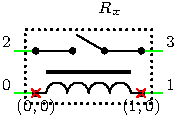
\includegraphics{relayInfo}
\caption{Example of use of relay}
\label{relayInfo} %Inserire sempre dopo caption
\end{figure}

\begin{figure}[h]
\centering
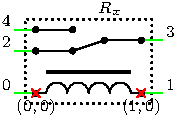
\includegraphics{relaySPDTInfo}
\caption{Example of use of relay SPDT}
\label{relaySPDTInfo} %Inserire sempre dopo caption
\end{figure}

\begin{figure}[h]
\centering
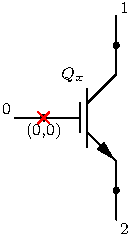
\includegraphics{igbtInfo}
\caption{Example of use of igbt}
\label{igbtrInfo} %Inserire sempre dopo caption
\end{figure}

\begin{figure}[h]
\centering
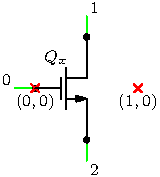
\includegraphics{mosInfo}
\caption{Example of use of MOS}
\label{mosInfo} %Inserire sempre dopo caption
\end{figure}

\begin{figure}[h]
\centering
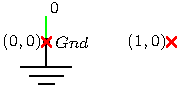
\includegraphics{gndPowerInfo}
\caption{Example of use of power ground symbol}
\label{gndPowerInfo} %Inserire sempre dopo caption
\end{figure}

\begin{figure}[h]
\centering
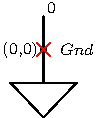
\includegraphics{gndSignalInfo}
\caption{Example of use of signal ground symbol}
\label{gndSignalInfo} %Inserire sempre dopo caption
\end{figure}

\end{document}